\documentclass[a4paper,12pt]{article}


%%% Работа с русским языком
\usepackage{cmap}					% поиск в PDF
\usepackage{mathtext} 				% русские буквы в формулах
\usepackage[T2A]{fontenc}			% кодировка
\usepackage[utf8]{inputenc}			% кодировка исходного текста
\usepackage[english,russian]{babel}	% локализация и переносы
\usepackage{indentfirst}
\frenchspacing

\newcommand{\vyp}{\ensuremath{\hookrightarrow}}
\renewcommand{\epsilon}{\ensuremath{\varepsilon}}
\renewcommand{\phi}{\ensuremath{\varphi}}
\renewcommand{\kappa}{\ensuremath{\varkappa}}
\renewcommand{\le}{\ensuremath{\leqslant}}
\renewcommand{\leq}{\ensuremath{\leqslant}}
\renewcommand{\ge}{\ensuremath{\geqslant}}
\renewcommand{\geq}{\ensuremath{\geqslant}}
\renewcommand{\emptyset}{\varnothing}
\newcommand{\Ra}{\ensuremath{\Rightarrow}}
\newcommand{\ra}{\ensuremath{\rightarrow}}
\newcommand{\LRa}{\ensuremath{\Leftrightarrow}}
\newcommand{\tbf}{\textbf}
\newcommand{\ov}{\ensuremath{\overline}}
\newcommand{\CC}{\ensuremath{\mathbb{C}}}
\newcommand{\RR}{\ensuremath{\mathbb{R}}}
\newcommand{\NN}{\ensuremath{\mathbb{N}}}
\newcommand{\QQ}{\ensuremath{\mathbb{Q}}}
\newcommand{\ZZ}{\ensuremath{\mathbb{Z}}}

%%% Дополнительная работа с математикой
\usepackage{amsmath,amsfonts,amssymb,amsthm,mathtools} % AMS
\usepackage{icomma} % "Умная" запятая: $0,2$ --- число, $0, 2$ --- перечисление

%% Номера формул
%\mathtoolsset{showonlyrefs=true} % Показывать номера только у тех формул, на которые есть \eqref{} в тексте.
%\usepackage{leqno} % Нумереация формул слева

%% Свои команды
\DeclareMathOperator{\sgn}{\mathop{sgn}}

%% Перенос знаков в формулах (по Львовскому)
\newcommand*{\hm}[1]{#1\nobreak\discretionary{}
{\hbox{$\mathsurround=0pt #1$}}{}}



%%% Работа с картинками
\usepackage{graphicx}  % Для вставки рисунков
\graphicspath{{images/}{images2/}}  % папки с картинками
\setlength\fboxsep{3pt} % Отступ рамки \fbox{} от рисунка
\setlength\fboxrule{1pt} % Толщина линий рамки \fbox{}
\usepackage{wrapfig} % Обтекание рисунков текстом

%%% Работа с таблицами
\usepackage{array,tabularx,tabulary,booktabs} % Дополнительная работа с таблицами
\usepackage{longtable}  % Длинные таблицы
\usepackage{multirow} % Слияние строк в таблице

%%% Теоремы
\theoremstyle{plain} % Это стиль по умолчанию, его можно не переопределять.
\newtheorem{theorem}{Теорема}[section]
\newtheorem{proposition}[theorem]{Утверждение}
 
\theoremstyle{definition} % "Определение"
\newtheorem{corollary}{Следствие}[theorem]
\newtheorem{problem}{Задача}[section]
 
\theoremstyle{remark} % "Примечание"
\newtheorem*{nonum}{Решение}

%%% Программирование
\usepackage{etoolbox} % логические операторы

%%% Страница
\usepackage{extsizes} % Возможность сделать 14-й шрифт
\usepackage{geometry} % Простой способ задавать поля
	\geometry{top=20mm}
	\geometry{bottom=20mm}
	\geometry{left=5mm}
	\geometry{right=15mm}
 %
\usepackage{fancyhdr} % Колонтитулы
 	\pagestyle{fancy}
 	\renewcommand{\headrulewidth}{1pt}  % Толщина линейки, отчеркивающей верхний колонтитул
%\fancypagestyle{firstpage}{
	\rhead{\large{Исыпов Илья}}
%}
% 	\lfoot{Нижний левый}
% 	\rfoot{\large{Рябых Владислав, Б05-905}}
% 	\rhead{Верхний правый]}
% 	\chead{Верхний в центре}
 	\lhead{\large{Рябых Владислав}}
%	\cfoot{Нижний в центре} % По умолчанию здесь номер страницы

\usepackage{setspace} % Интерлиньяж
\onehalfspacing % Интерлиньяж 1.5
%\doublespacing % Интерлиньяж 2
%\singlespacing % Интерлиньяж 1

\usepackage{lastpage} % Узнать, сколько всего страниц в документе.

\usepackage{soul} % Модификаторы начертания

\usepackage{hyperref}
\usepackage[usenames,dvipsnames,svgnames,table,rgb]{xcolor}
\hypersetup{				% Гиперссылки
    unicode=true,           % русские буквы в раздела PDF
    pdftitle={Заголовок},   % Заголовок
    pdfauthor={Автор},      % Автор
    pdfsubject={Тема},      % Тема
    pdfcreator={Создатель}, % Создатель
    pdfproducer={Производитель}, % Производитель
    pdfkeywords={keyword1} {key2} {key3}, % Ключевые слова
    colorlinks=true,       	% false: ссылки в рамках; true: цветные ссылки
    linkcolor=red,          % внутренние ссылки
    citecolor=black,        % на библиографию
    filecolor=magenta,      % на файлы
    urlcolor=cyan           % на URL
}

\usepackage{csquotes} % Еще инструменты для ссылок

%\usepackage[style=authoryear,maxcitenames=2,backend=biber,sorting=nty]{biblatex}

\usepackage{multicol} % Несколько колонок

\usepackage{tikz} % Работа с графикой
\usepackage{pgfplots}
\usepackage{pgfplotstable}

\usepackage{caption}
\long\def\comment{}
\setlength{\abovecaptionskip}{7pt}
\setlength{\belowcaptionskip}{7pt}
\usepackage{makecell}
\mathtoolsset{showonlyrefs}

% Allow line breaks with \\ in specialcells
\newcommand{\specialcell}[2][c]{%
	\begin{tabular}[#1]{@{}c@{}}#2\end{tabular}
}

\begin{document}

\begin{titlepage}
	\begin{center}
		
		\textsc{\LARGE Московский\\[-0.2cm]Физико-Технический Институт\\[0.1cm]\large (национальный исследовательский университет)}\\[1.5cm] 
		
	
\includegraphics[width=0.3\textwidth]{hv_s_no_bg.png}~\\[1cm]

	\textsc{\Large Оптика. \\ Лабораторный практикум. }\\[0.2cm]

	% Title
	\HRule \\[0.4cm]
	{ \LARGE \bfseries Лабораторная работа № 4.3.2 \\ Дифракция света на ультразвуковой волне в жидкости. \\[0.4cm] }

	\HRule \\[1.5cm]
		
		% Author and supervisor
		\noindent
		\begin{minipage}{0.4\textwidth}
			\begin{flushleft} \large
			\end{flushleft}
		\end{minipage}%
		\begin{minipage}{0.4\textwidth}
			\begin{flushright} \large
			\end{flushright}
		\end{minipage}
		
		
		\large{\begin{flushright}
				\vfill
				\textbf{Выполнили}:\\
				\textbf{Рябых Владислав,\\}
				\textbf{Исыпов Илья\\}
				\textbf{группа Б05-905}
		\end{flushright}}
		
		
		{\large \today}\\
		
		
	\end{center}
\end{titlepage}

\subsubsection*{Цель работы:} изучение дифракции света на синусоидальной акустической решетке и
наблюдение фазовой решетки методом темного поля.

\subsubsection*{Оборудование:} оптическая скамья, осветитель, два длиннофокусных объектива, кювета с жидкостью, кварцевый излучатель с микрометрическим винтом, генератор звуковой частоты, линза, вертикальная нить на рейтере, микроскоп.

\section*{Теория}

При прохождении ультразвуковой волны через жидкость в ней возникают периодические неоднородности коэффициента преломления, создается фазовая решетка, которую мы считаем неподвижной ввиду малости скорости звука относительно скорости света. Показатель
преломления $n$ изменяется по закону:

\begin{equation}\label{}
n = n_0 (1 + m \cos \Omega x)
\end{equation}

Здесь $ \Omega = 2 \pi / \Lambda $ --- волновое число для ультразвуковой волны, $ m $ --- глубина модуляции $ n $ $ (m \ll 1 $).

Положим фазу $ \phi $ колебаний световой волны на передней стенке кюветы равной нулю, тогда на задней поверхности она равна:

\begin{equation}\label{}
\phi  = k n L = \phi_0 (1 + m \cos \Omega x)
\end{equation}

Здесь $ L $ --- толщина жидкости в кювете, $ k = 2 \pi / \lambda $ --- волновое число для света.

После прохождения через кювету световое поле есть совокупность плоских волн, распространяющихся под углами $ \theta $, соответствующими максимумам в дифракции Фраунгофера:

\begin{equation}\label{eq:1}	
\Lambda \sin \theta_m = m \lambda
\end{equation}

Этот эффект проиллюстрирован на рисунке \ref{diff}.
\begin{figure}[bhtp!]
	\centering	
	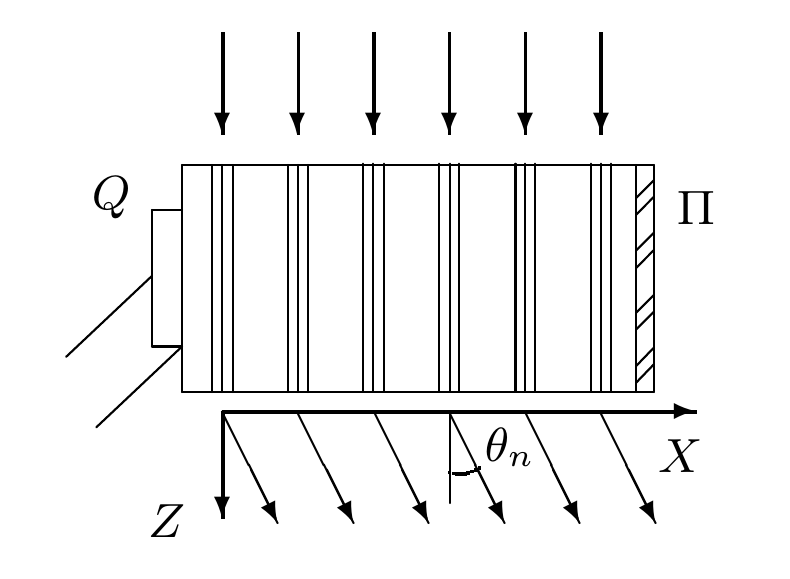
\includegraphics[width=0.36\textwidth]{difraction.png}
	\caption{Дифракция световых волн на акустической решетке}
	\label{diff}
\end{figure}

Зная положение дифракционных максимумов, по формуле \eqref{eq:1} легко определить длину ультразвуковой волны, учитывая малость $ \theta $: $ \sin \theta \approx \theta \approx l_m /F  $, где $ l_m $ --- расстояние от нулевого до последнего видимого максимума, $ F $ --- фокусное расстояние линзы. Тогда получим:

\begin{equation}\label{eq:2}
\Lambda = m \lambda F/ l_m 
\end{equation}
Скорость ультразвуковых волн в жидкости, где $ \nu $ --- частота колебаний излучателя:

\begin{equation}\label{eq:3}
v = \Lambda \nu 
\end{equation}

\section*{Ход работы}

\subsection*{Определение скорости ультразвука по дифракционной картине}

Схема установки приведена на рисунке \ref{shema1}. Источник света Л через светофильтр Ф и конденсор К освещает вертикальную щель $S$, находящуюся в фокусе объектива $O_1$. После объектива параллельный световой пучок проходит через кювету С перпендикулярно акустической решетке, и дифракционная картина собирается в фокальной плоскости объектива $O_2$, наблюдается при помощи микроскопа М.
	
Предварительную настройку установки произведем в соответствии с инструкцией с зеленым фильтром, далее в работе используется красный.
	
\begin{figure}[bhtp!]
	\centering	
	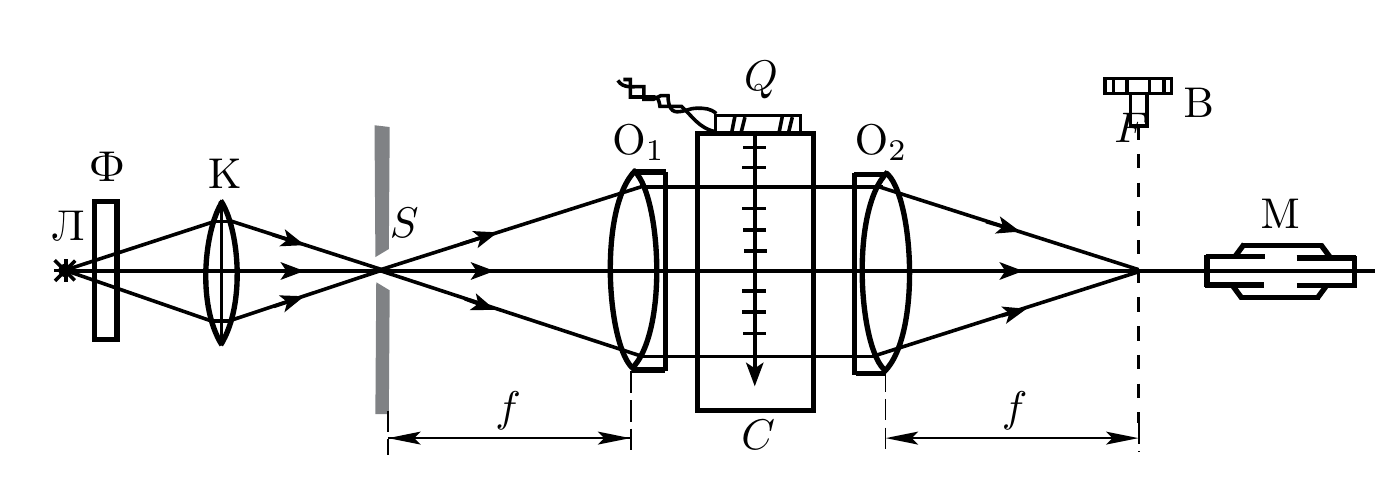
\includegraphics[width=0.7\textwidth]{shema1.png}
	\caption{Схема для наблюдения дифракции на акустической решетке}
	\label{shema1}
\end{figure}
	
Параметры установки: фокусное расстояние объектива $  O_2  $ $ F = 30 $ см, одно деление винта микроскопа составляет 4 мкм, погрешность измерений примем равной  $ \sigma = $ 2 деления, или 8 мкм.
	
Исследуем изменения дифракционной картины на зеленом свете. При увеличении частоты УЗ-генератора и приближении к 1,1 МГц проявляется дифракционная решетка: расстояние между максимумами растет.
	
Измерим положения $ x_m $ дифракционных максимумов с помощью микроскопического винта для четырех частот. Результаты измерений занесены в таблицы \ref{tab:1}, \ref{tab:2}, \ref{tab:3}, \ref{tab:4}. На основе каждой таблицы построены графики зависимости $ x_m (m) $, они изображены на рисунках \ref{gr1}, \ref{gr2}, \ref{gr3}, \ref{gr4}. Коэффициенты углов наклона прямых $b$ для всех зависимостей сведены в таблицу \ref{tab:5}. 
	
\begin{table}[bhtp!]
	\centering
	
	\begin{tabular}{|c|c|c|c|c|c|c|c|}
		\hline
		$m$&-3&-2&-1&0&1&2&3\\
		\hline
		$x_m$, дел&2.85&3.21&3.62&4.0&4.37&4.72&5.17\\
		\hline
		$\Delta x_m$, мкм&-460&-316&-152&0&148&288&468\\
		\hline
	\end{tabular}
	
	\caption{Измерение координаты $ m $-ого максимума $ x_m $ при частоте генератора $ \nu = $ 1.076 МГц}
	\label{tab:1}
\end{table}	
	
\begin{figure}[bhtp!]
	\centering
	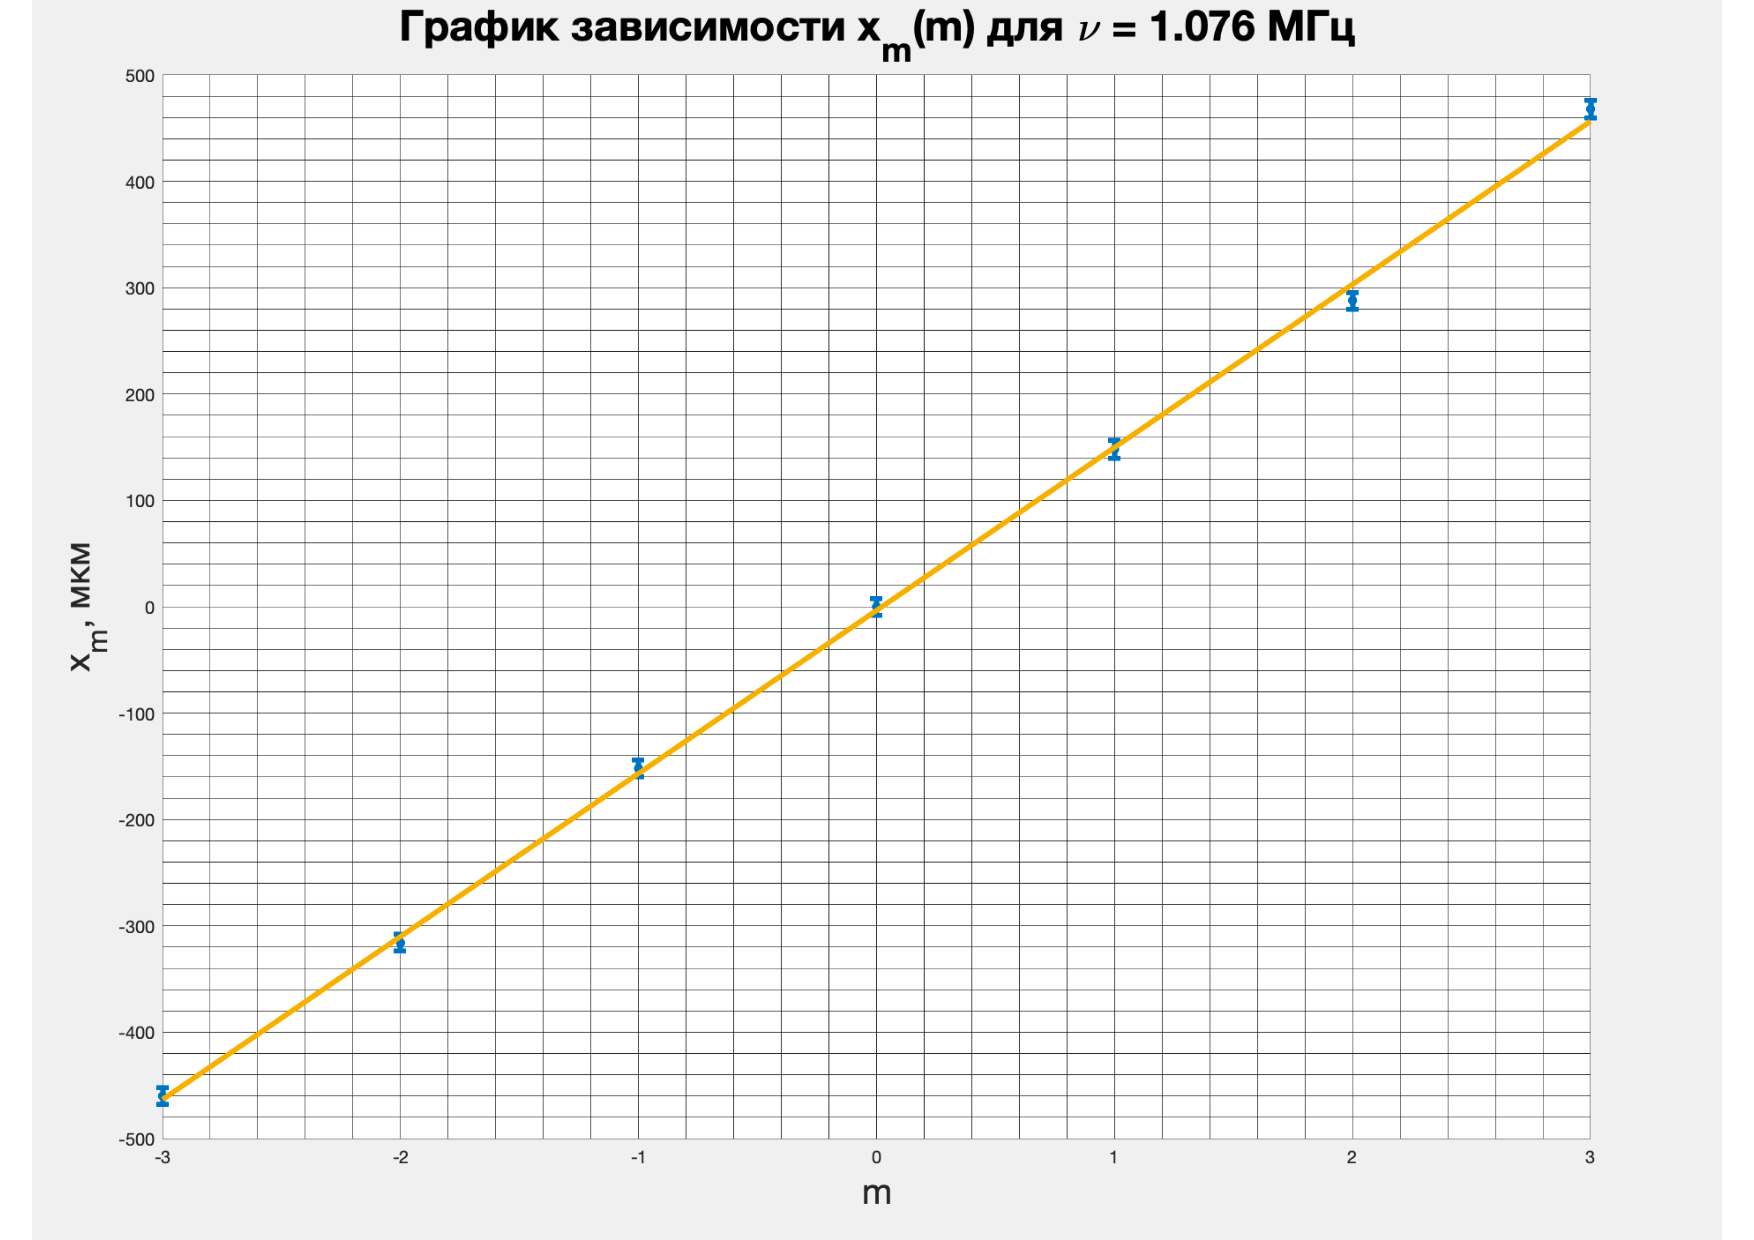
\includegraphics[width=0.63\linewidth]{gr1.pdf}
	\caption{График зависимость $ x_m(m)$ при частоте генератора $\nu = 1.076$ МГц}
	\label{gr1}
\end{figure}
	
\begin{table}[bhtp!]
	\centering
	
	\begin{tabular}{|c|c|c|c|c|c|c|c|}
		\hline
		$m$ &-3&-2&-1&0&1&2&3\\
		\hline
		$x_m$, дел&2.84&3.20&3.63&4.0&4.35&4.71&5.23\\
		\hline
		$\Delta x_m$, мкм&-464&-320&-148&0&140&284&492\\
		\hline
	\end{tabular}	
	\caption{Измерение координаты $ m $-ого максимума $ x_m $ при частоте генератора $ \nu = 1.089$ МГц}
	\label{tab:2}
\end{table}	
	
\begin{figure}[bhtp!]
	\centering
	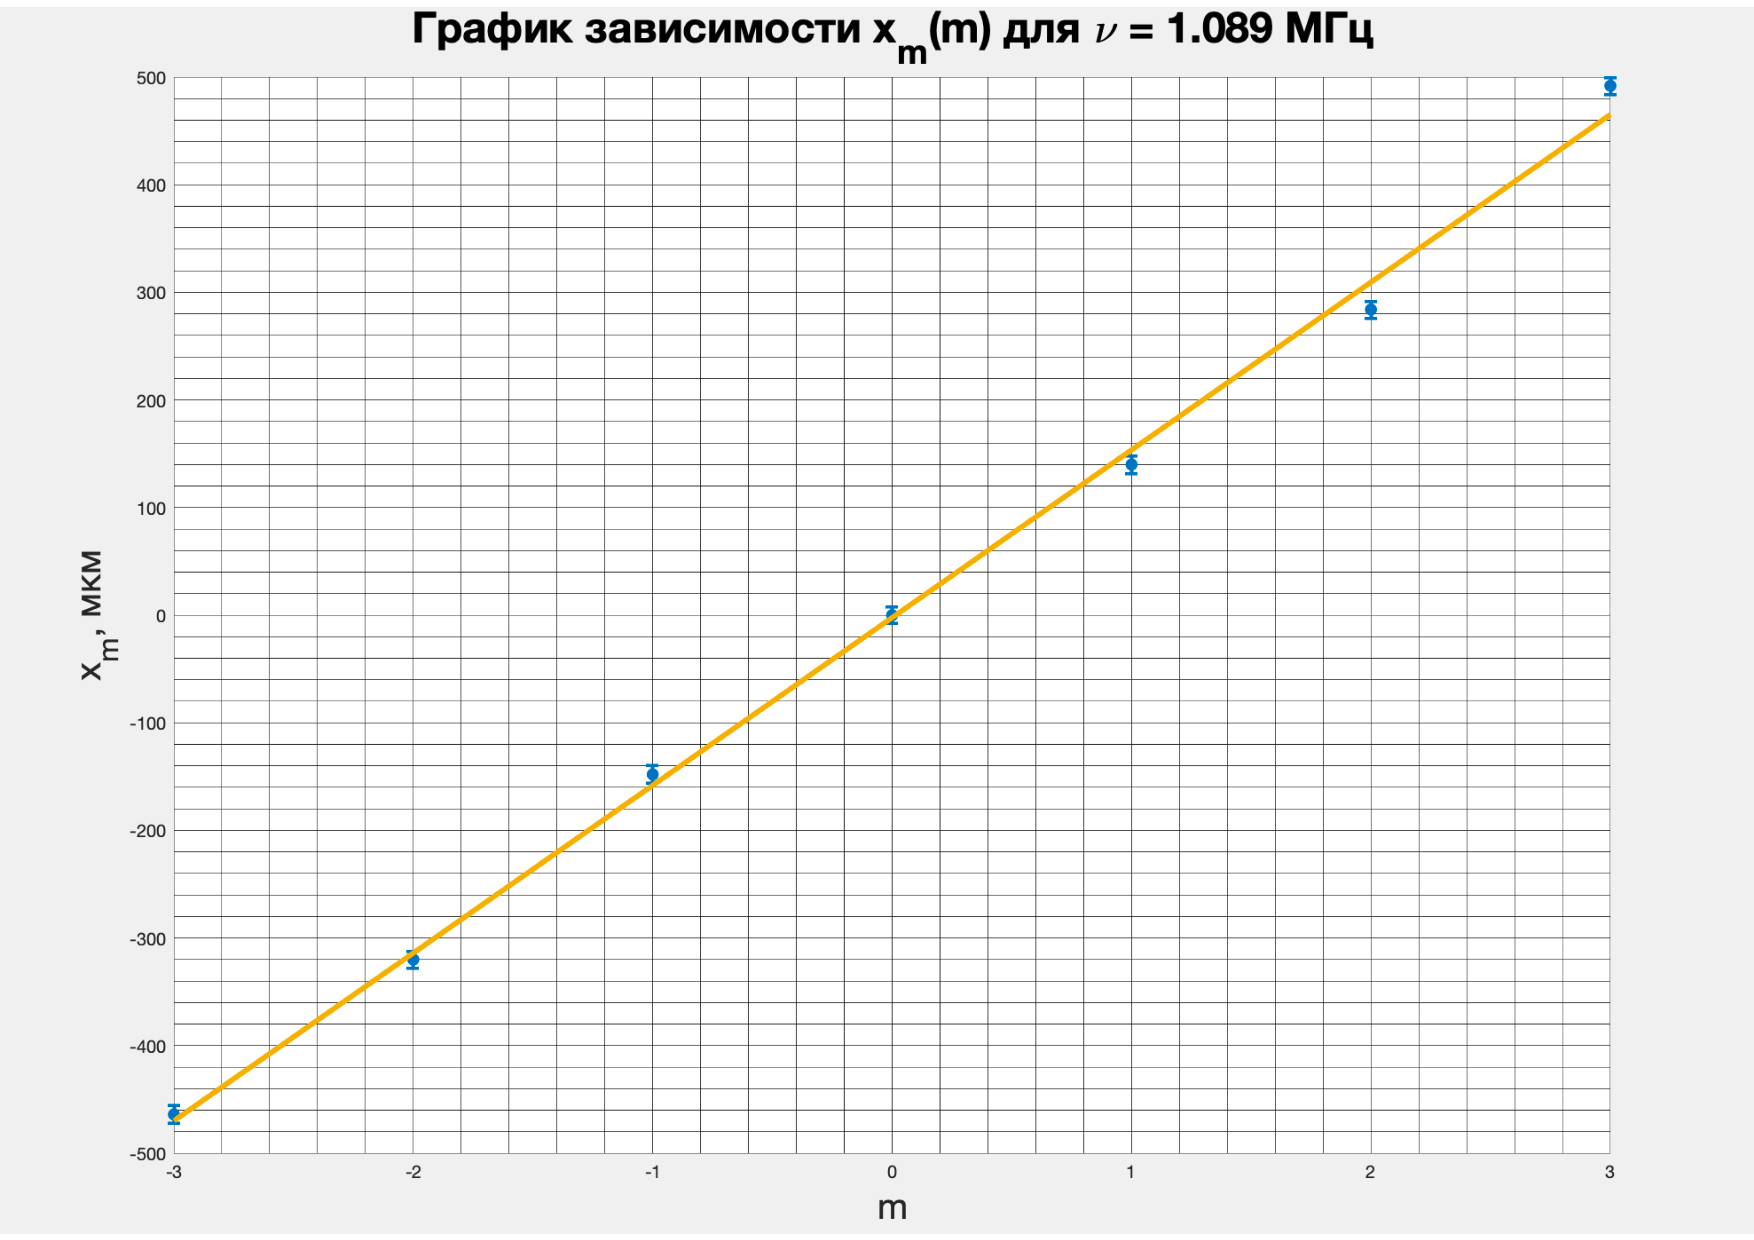
\includegraphics[width=0.63\linewidth]{gr2.pdf}
	\caption{График зависимость $  x_m(m) $ при частоте генератора $ \nu = 1.089$ МГц}
	\label{gr2}
\end{figure}
	
\begin{table}[bhtp!]
	\centering
	
	\begin{tabular}{|c|c|c|c|c|c|c|c|}
		\hline
		$m$&-3&-2&-1&0&1&2&3\\
		\hline
		$x_m$, дел&2.9&3.2&3.7&4.0&4.43&4.8&5.3\\
		\hline
		$\Delta x_m$, мкм&-440&-304&-120&0&172&320&520\\
		\hline
	\end{tabular}
	
	\caption{Измерение координаты $ m $-ого максимума $ x_m $ при частоте генератора $ \nu =  1.165$ МГц}
	\label{tab:3}
\end{table}	
	
\begin{figure}[bhtp!]
	\centering
	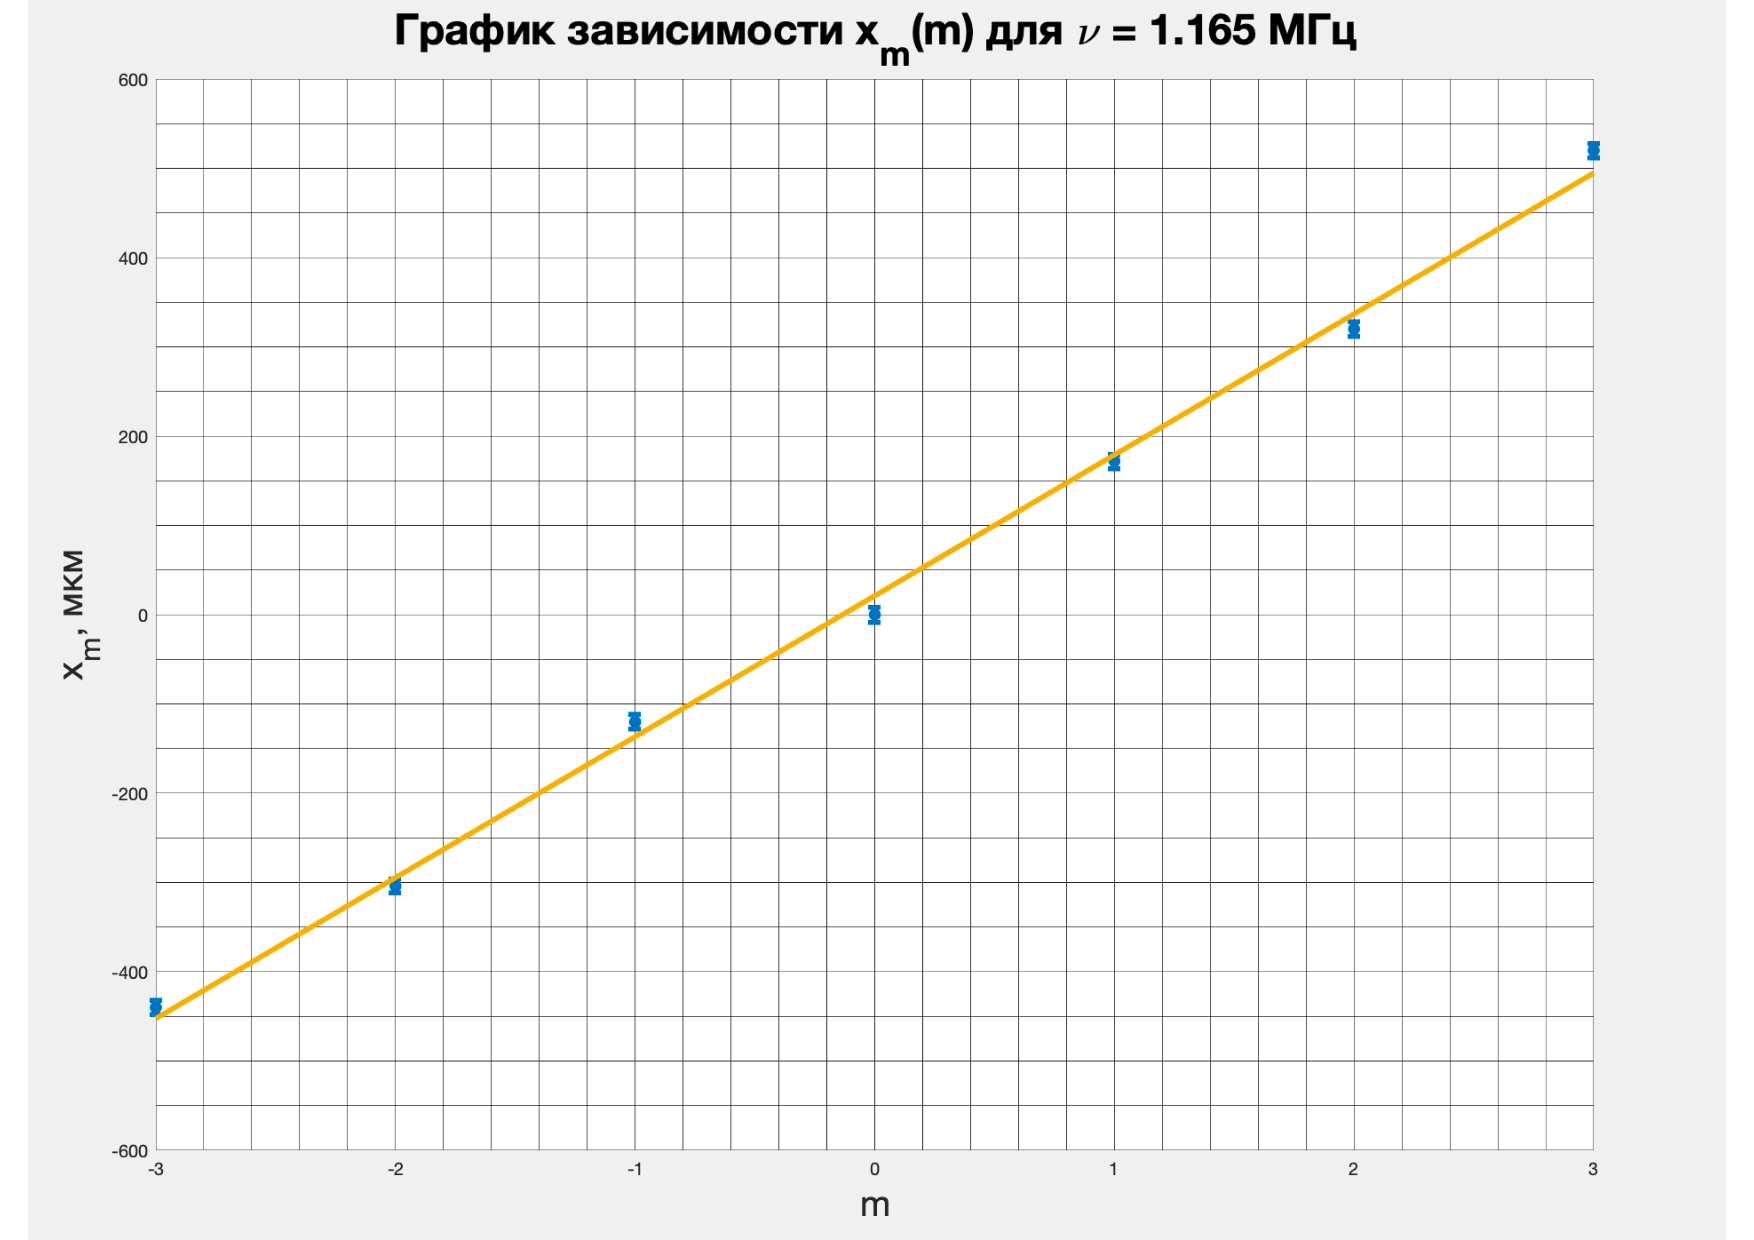
\includegraphics[width=0.63\linewidth]{gr3.pdf}
	\caption{График зависимость $x_m(m) $ при частоте генератора $\nu = 1.165$ МГц}
	\label{gr3}
\end{figure}
	
\begin{table}[bhtp!]
	\centering
	
	\begin{tabular}{|c|c|c|c|c|c|c|c|}
		\hline
		$m$&-3&-2&-1&0&1&2&3\\
		\hline
		$x_m$, дел&2.54&3.1&3.7&4.0&4.45&5.06&5.75\\
		\hline
		$\Delta x_m$, мкм&-584&-360&-120&0&180&424&700\\
		\hline
	\end{tabular}
	
	\caption{Измерение координаты $ m $-ого максимума $ x_m $ при частоте генератора $ \nu = $ 1.289 МГц}
	\label{tab:4}
\end{table}	
	
\begin{figure}[bhtp!]
	\centering
	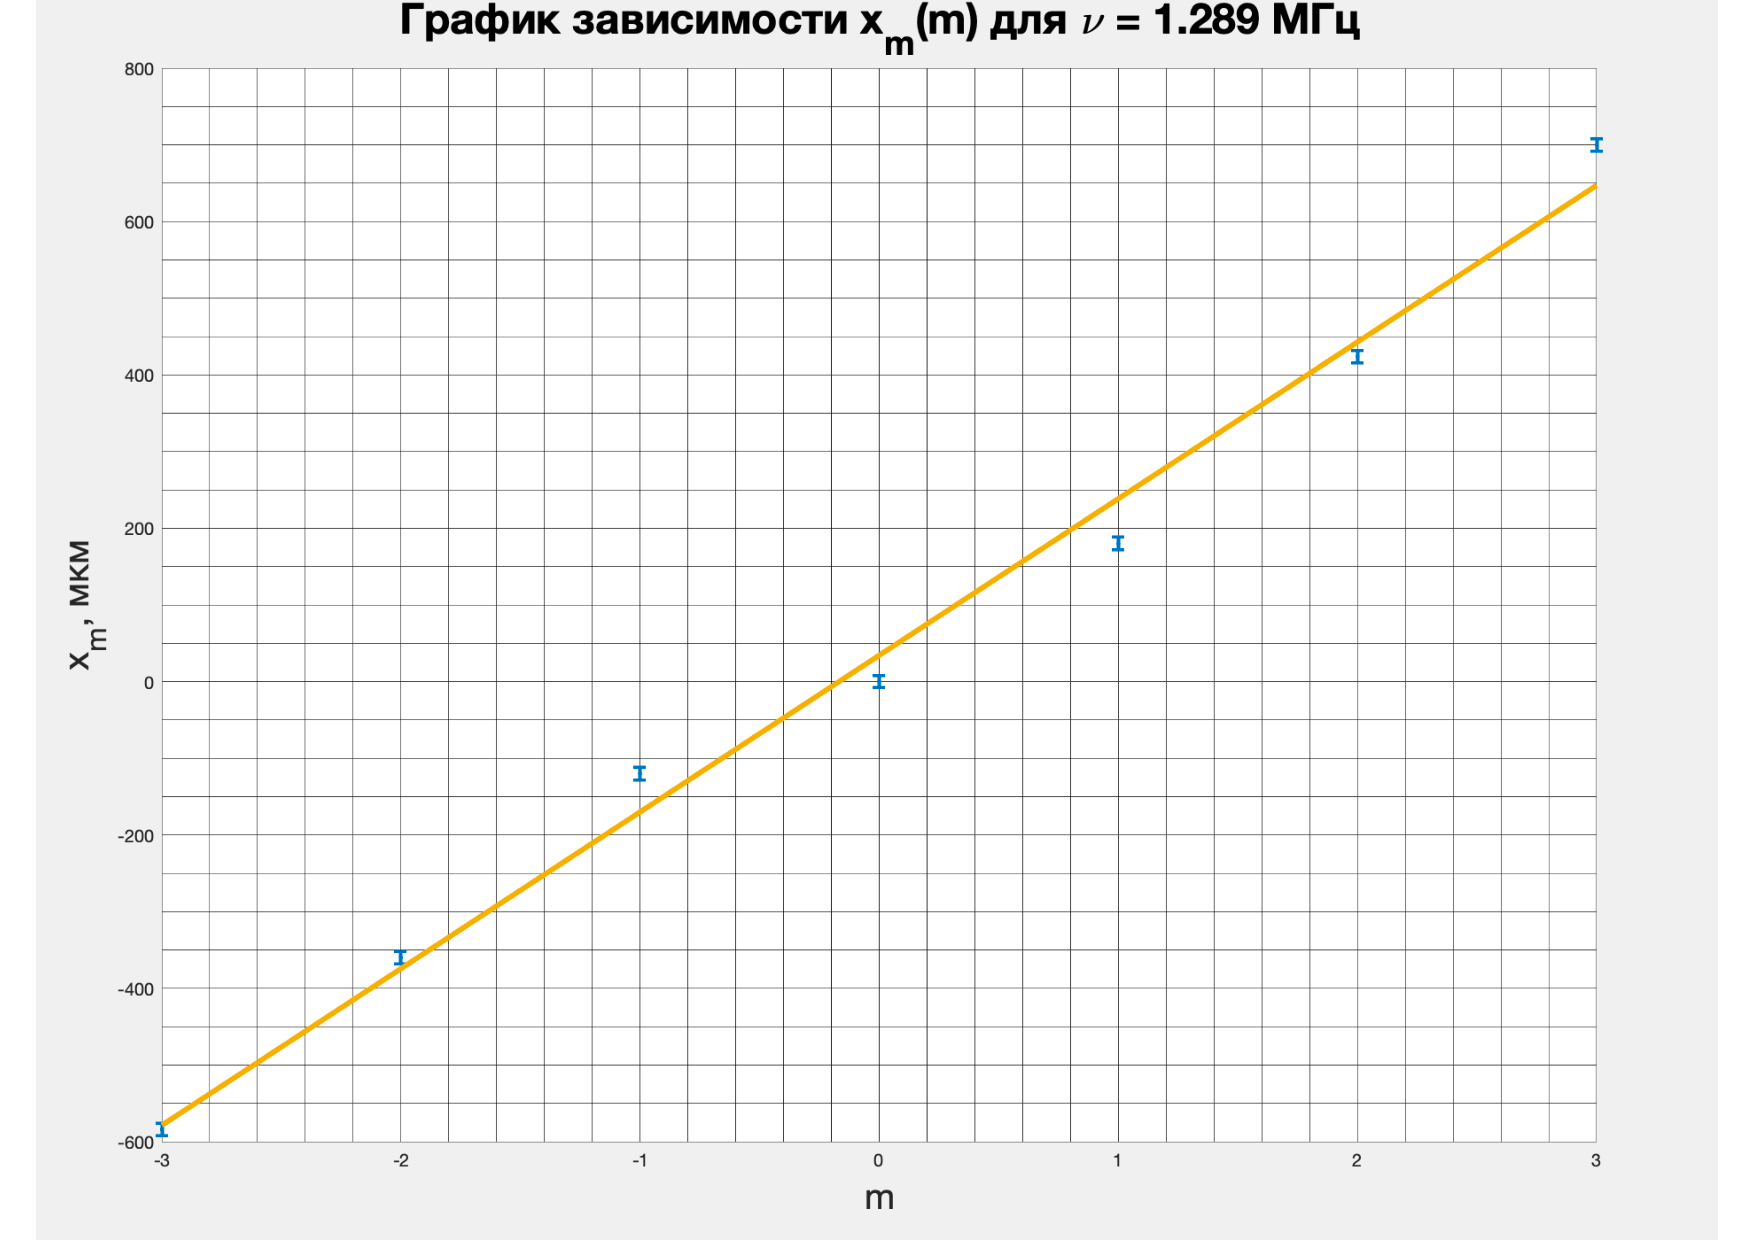
\includegraphics[width=0.63\linewidth]{gr4.pdf}
	\caption{График зависимость$  x_m(m) $ при частоте генератора $ \nu = $ 1.289 МГц}
	\label{gr4}
\end{figure}
	
\begin{table}[bhtp!]
	\centering
	
	\begin{tabular}{|c|c|c|c|c|c|}
		\hline
		$\nu$, МГц& $b$, мкм& $\Lambda$, мкм&$\Delta \Lambda$, мкм&$v$, м/с&$\Delta v$, м/с \\ \hline
		1.076 & 153.29 & 1346 & 15  & 1448 & 17  \\ \hline
		1.089 & 155.86 & 1358 & 13  & 1479 & 14  \\ \hline
		1.165 & 157.86 & 1212 & 12  & 1411 & 13  \\ \hline
		1.289 & 204.29 & 1079 & 19  & 1391 & 26  \\ \hline
	\end{tabular}
	
	\caption{Вычисление длины ультразвуковой волны $ \Lambda $ и скорости её распространения в воде $v$}
	\label{tab:5}
\end{table}	
	
	
Ошибка при определении $ \Lambda $ и $ v $ не превышает 2\%. Согласно справочным данным, при комнатной температуре скорость ультразвуковой волны в воде составляет примерно 1490 м/с. Значения, полученные экспериментально, с достаточной точностью соотносятся с ними.

\subsection*{Изменение характера поляризации света при наличии внешнего поля}

Для наблюдения акустической решетки используется метод темного поля, который заключается в устранении центрального дифракционного максимума с помощью непрозрачного экрана. Схема установки показана на рисунке \ref{shema2}.

\begin{figure}[bhtp!]
	\centering	
	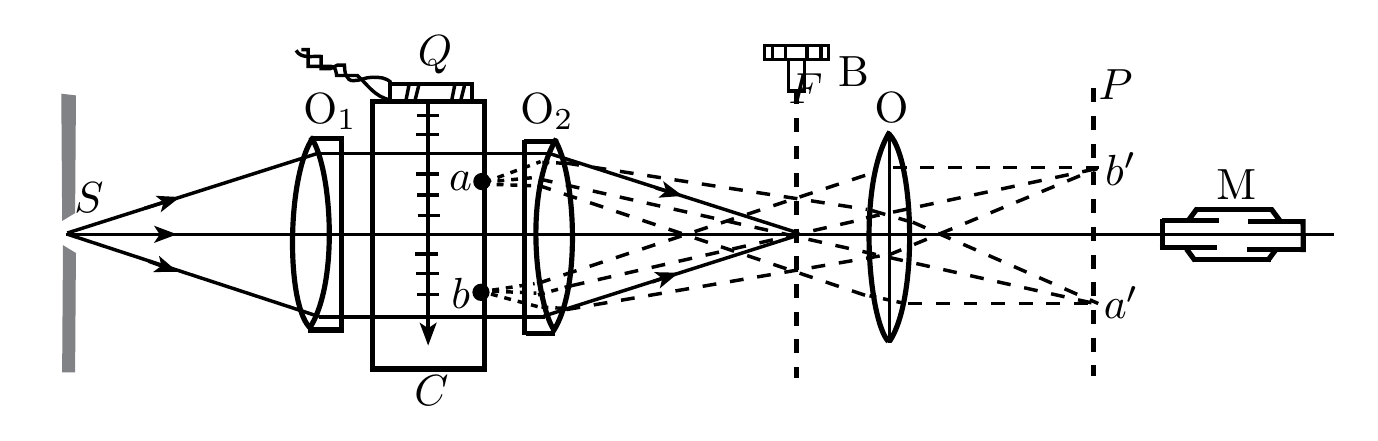
\includegraphics[width=0.7\textwidth]{shema2.png}
	\caption{Схема для наблюдения дифракции методом темного поля}
	\label{shema2}
\end{figure}

Приставим к задней стенке (для светового луча) кюветы стеклянную пластинку с миллиметровыми делениями; сфокусируем микроскоп на изображение пластинки. Определим цену деления окулярной шкалы микроскопа, совместив ее с миллиметровыми делениями: в 6 делениях миллиметровой шкалы убирается 100 маленьких делений окулярной. Значит, цена деления окулярной шкалы: $ C = $ 0,06 мм.

Без применения метода темного поля звуковая решетка не наблюдается. Закроем нулевой максимум горизонтальной нитью. Таким образом, осевая составляющая фазово-модулированной волны поглощается, а боковые остаются без изменения. Получившееся поле: 

\begin{equation}\label{}
f(x) = \dfrac{im}{2} e^{i\Omega x} +  \dfrac{im}{2} e^{-i\Omega x} = im \cos \Omega x \Ra I(x) = m^2 \cos ^2 \Omega x = m^2 \dfrac{1 + \cos ^2 2 \Omega x}{2}
\end{equation}

Отсюда получаем, что расстояние между темными полосами есть $ \Lambda/2 $.

Проведем измерение длины ультразвуковой волны, приняв ошибку равной цене деления окулярной шкалы. В таблице \ref{tab:6} содержатся количество маленьких делений окулярной шкалы N (цена деления $ C = 0.06 $), соответствующее $ n $ темным полосам акустической решетки.
Формулы для расчета длины волны ультразвука $ \Lambda $ и скорости распространения $ v $ в воде:
\begin{equation}\label{}
\Lambda/2  = NC/(n - 1),  \qquad v = \nu\Lambda
\end{equation}

Расчеты также приведены в таблице \ref{tab:6}. Ошибка при таком определении скорости звука больше, чем в первой части работы, и
составляет около 5\%. Сами значения тоже получились больше.


\begin{table}[bhtp!]
	\centering
	
	\begin{tabular}{|c|c|c|c|c|c|c|c|c|c|}
		\hline
		$\nu$, Мгц& \specialcell{Количество делений \\ шкалы окуляра $N$}&\specialcell{Количество темных полос \\ акустической решетки $n$}&$\Lambda$, мм&$v$, м/с&$\Delta v$, м/с\\
		\hline
		1.220&150&15&1.29&1570&70\\
		\hline
		1.259&150&16&1.20&1510&80\\
		\hline
		1.271&175&18&1.24&1570&80\\
		\hline
	\end{tabular}
	
	
	\caption{Вычисление длины ультразвуковой волны $ \Lambda $ и скорости распространения ее в воде $ v $ методом темного поля}
	\label{tab:6}
\end{table}	

\section*{Вывод}

В работе были изучены дифракция света на синусоидальной акустической решётке и фазовая решётка, полученная методом тёмного поля. Также были рассчитаны длина волны ультразвука и скорость его распространения в воде.
\end{document}